\documentclass[12pt,a4paper]{article}
\usepackage[utf8]{inputenc}
\usepackage[english]{babel}
\usepackage{amsmath}
\usepackage{amsfonts}
\usepackage{amssymb}
\usepackage{graphicx}

\title{OPTICS in Clean}
\date{August 18, 2013}
\author{Patrick Uiterwijk\\Robin Smit}

\begin{document}

\maketitle
\clearpage

\begin{abstract}
OPTICS (Ordering Points To Identify The Clustering Structure) is an algorithm that may be used as a pre-processing method in order to find clusters in spatial data.\\
The algorithm takes spatial data as input and returns a linear ordering of that data. In this ordering, data points that are spatially closest become neighbours.\\
The data points in the result are paired with additional specific information about spatial closeness to such a point's neighbours. This information may be used to determine an actual clustering of the given data.

This article will give an implementation, analysis and a test case for the OPTICS algorithm written in the functional programming language Clean.
\end{abstract}
\clearpage

\tableofcontents
\clearpage

\section{Previous work}
The interesting thing about this project is that a lot of descriptions can be found on the internet. All of these, however, target imperative implementations. What we will try to do is to provide a functional implementation of the OPTICS algorithm for clustering.

\clearpage
\section{Method}
As for many programs, it's generally a good idea to make sure one has a clear understanding of what the program to be implemented should accomplish, and the way in which that result should be achieved.

\subsection{Test case}
We thought of a test case that would provide us with an input allowing us to easily see the results of our algorithm. We took a diagram from the web and extracted it's color values. Our functional OPTICS algorithm should then be able to cluster these values into main colors, generating an image that looks like the original one. Below is an example of such a diagram and it's original color plot:\\

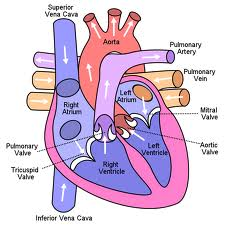
\includegraphics[scale=0.6]{img/diagram.png}
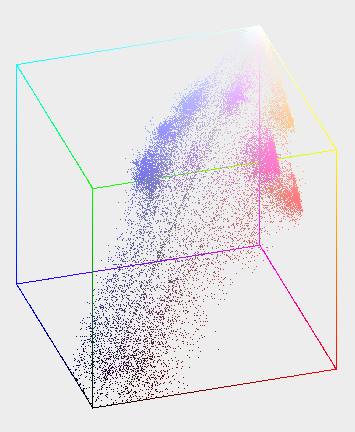
\includegraphics[scale=0.6]{img/colorplot.png}
\\
\\
One can see clearly some clusters of the colors white, yellow, orange, as well as some shades of magenta and purple.

\subsection{General application}
If the algorithm is to run correctly these pixels should be clustered with other pixels of their approximate shade. These clusters could then be averaged for a color. When pixels are then translated back onto a two-dimensional plane (an image), that new image will contain significantly less colors and can be stored more efficiently.

\clearpage
\section{Main results}
We have implemented the OPTICS algorithm in Clean – a functional language. The program itself can be found in the appendix to this report. Following is a description of how the algorithm works.

\subsection{Data}
The input to our OPTICS algorithm will exist of a number of Vectors. Such a Vector is simply a list of real numbers. The full input (of type Data) is a collection of Vectors. Duplicates may exist within such a Data object.

\subsection{Distance}
First, what we need is a function that computes the distance between two points. We have chosen to work with the Euclidean 1-norm distance (also known as the Manhattan distance), because the triangle inequality holds for this norm and it is less computationally intensive than the 2-norm distance taught in high school.

\begin{equation}
d(x,y)=\sum_{i=1}^n |x_i-y_i|
\end{equation}

\clearpage
\section{Analysis}
Text body

\section{Evaluation}
\subsection{Project outcome}
Text body
\subsection{Expectations}
With respect to efficiency, we do not expect our implementation of the OPTICS algorithm to be better than existing 

\section{Future directions}
The algorithm as we have implemented it, executes on a collection of Vectors in a real vector space. This input could be generalized to Vectors of other vector spaces. One would have to generalize the Vector definition, and also define a matching function to calculate a proximity between any such two Vectors.

\clearpage
\section{Appendix}
The program
\end{document}
